\section{\textsc{Beilagensalat}}

\subsection*{Zutaten für 2 Portionen:}

\begin{tabular}{p{7.5cm} p{7.5cm}}
	& \\
	4Blätter Eichbergsalat & \sfrac{1}{2} Gurke \\
	2 Karotten & \sfrac{1}{4} Rettich
\end{tabular}

\subsection*{Serviervorschlag:}

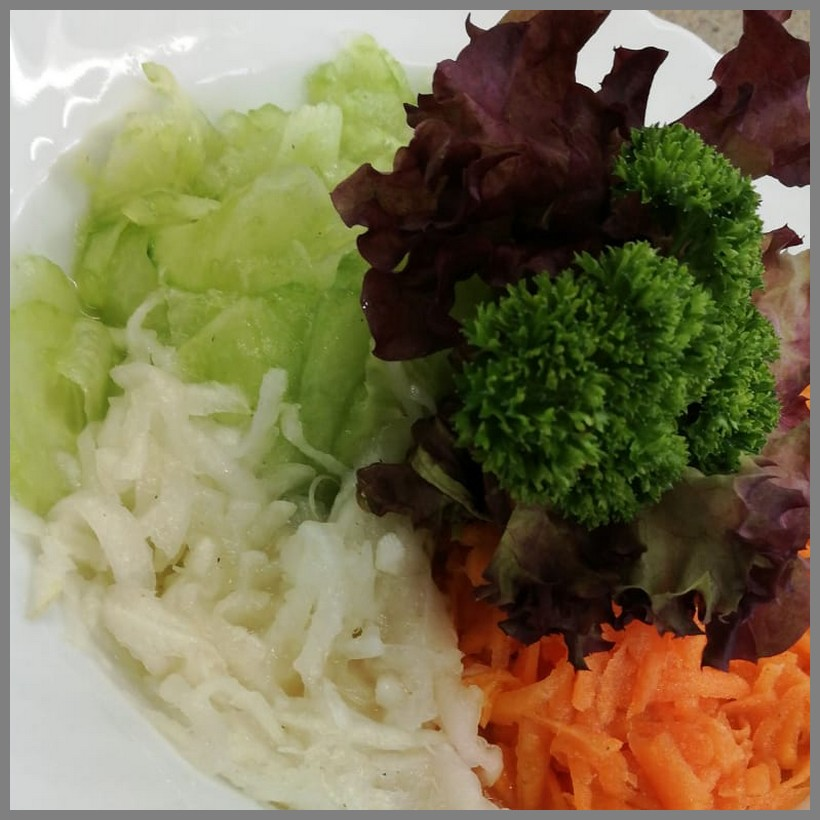
\includegraphics[width=\textwidth]{img/beilagensalat.jpeg} \cite{beilagensalat}

\subsection*{So geht's:}
\begin{tabular}{p{15cm}}
	\\
	Rettich, Karotten grob raspeln und die Gurke in dünne Streifen schneiden.\\
	Alles auf einem Teller anrichten.
\end{tabular}
